\documentclass{standalone}
\author{Quinten Bruynseraede}
\usepackage{tikz}
\usetikzlibrary{shapes}
\title{Tikz grafen}
\begin{document}\pagestyle{empty}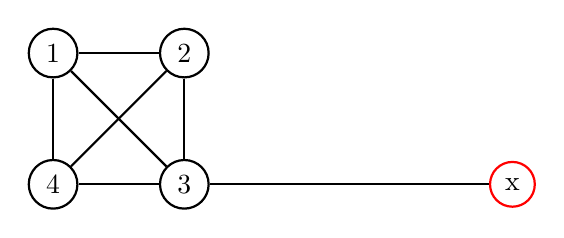
\begin{tikzpicture}\node[shape=circle,draw=black,align=center,line width=0.8pt] (0) at (1.6666666666666667,10.833333333333334) {1};
\node[shape=circle,draw=black,align=center,line width=0.8pt] (1) at (1.6666666666666667,9.166666666666666) {4};
\node[shape=circle,draw=black,align=center,line width=0.8pt] (2) at (3.3333333333333335,9.166666666666666) {3};
\node[shape=circle,draw=black,align=center,line width=0.8pt] (3) at (3.3333333333333335,10.833333333333334) {2};
\node[shape=circle,draw=red,align=center,line width=0.8pt] (4) at (7.5,9.166666666666666) {x};

\path [-,draw=black,line width=0.8pt] (0) edge node {} (1);
\path [-,draw=black,line width=0.8pt] (1) edge node {} (2);
\path [-,draw=black,line width=0.8pt] (2) edge node {} (3);
\path [-,draw=black,line width=0.8pt] (0) edge node {} (3);
\path [-,draw=black,line width=0.8pt] (0) edge node {} (2);
\path [-,draw=black,line width=0.8pt] (1) edge node {} (3);
\path [-,draw=black,line width=0.8pt] (2) edge node {} (4);
\end{tikzpicture}
\end{document}